\documentclass[tikz,border=10pt]{standalone}
\begin{document}
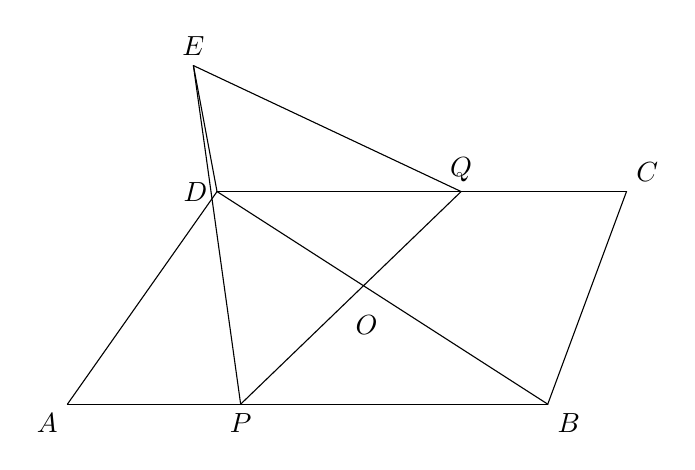
\begin{tikzpicture}[line cap=round,line join=round,scale=1]

% Coordinates
\coordinate (A) at (0,0);
\coordinate (P) at (2.2,0);
\coordinate (B) at (6.1,0);
\coordinate (D) at (1.9,2.7);
\coordinate (E) at (1.6,4.3);
\coordinate (Q) at (5.0,2.7);
\coordinate (C) at (7.1,2.7);
\coordinate (O) at (3.8,1.25);

% Outer boundary and main segments
\draw (A) -- (P) -- (B);
\draw (A) -- (D);
\draw (D) -- (E);
\draw (E) -- (Q);
\draw (D) -- (Q) -- (C);
\draw (B) -- (C);

% Interior segments
\draw (E) -- (P);
\draw (P) -- (Q);
\draw (D) -- (B);

% Labels
\node[below left] at (A) {$A$};
\node[below] at (P) {$P$};
\node[below right] at (B) {$B$};
\node[left] at (D) {$D$};
\node[above] at (E) {$E$};
\node[above] at (Q) {$Q$};
\node[above right] at (C) {$C$};
\node[below] at (O) {$O$};

\end{tikzpicture}
\end{document}
